\chapter{Data Exploration} \label{chap:data}

% This section will contain the exploration of the patient metadata, input data (peak strain values, and strain curves) and target variables. \bigskip
In this chapter the variability, distribution and type of data used in the assignment will be explored. 
The exploration is divided into three sections corresponding to the three main groups of variables: 
The \textit{patient meta-data}, the \textit{input variables} and the \textit{target variables}. 
The \textit{meta-data} is the data about the patients which is not used in the classification models, 
but can be used to give a description of the patient demographich which makes up the dataset. 
The \textit{input variables} are the variables that are inputed into the machine learning models in order to train them, 
and later used to make predictions about the patients' \textit{target variables}. 
The target variables are then variables that the models will be trained to predict. 
Target variables are used both in training to correct erroneus predictions that models make during training, and to evaluate the accuracy of the model after training. \bigskip

\section{Patient Meta-data} \label{sec:metadata}
The patient meta-data that will be considered in this section are age, gender, \acrfull{bmi} and blood pressure.

\begin{figure}
    \begin{center}
    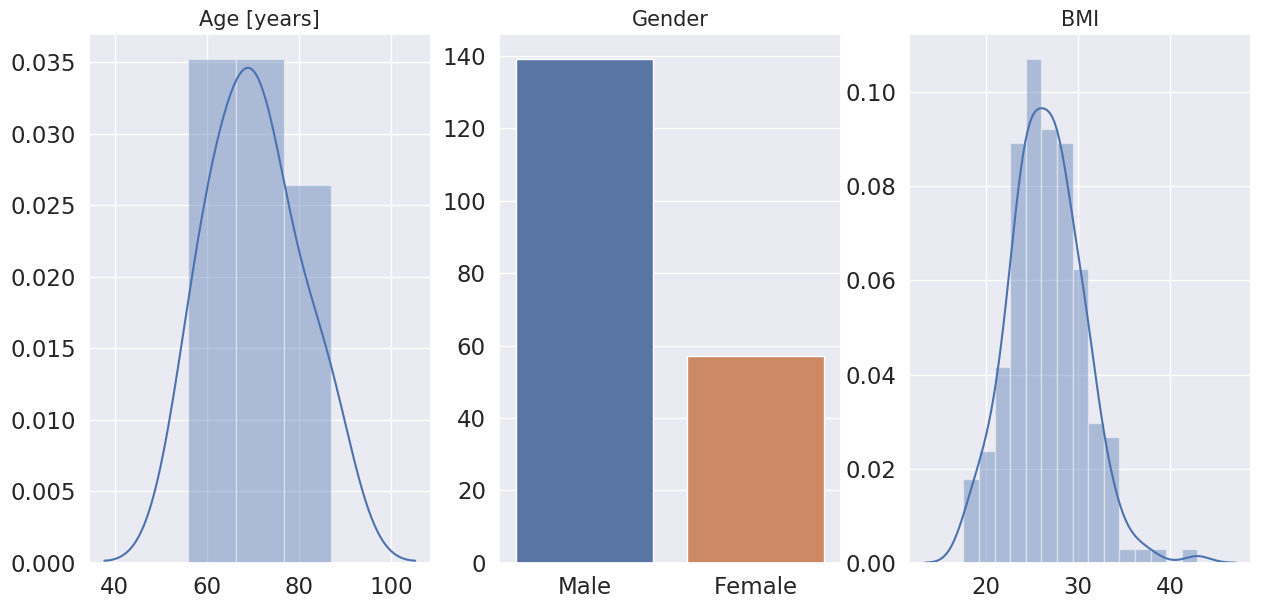
\includegraphics[width=\textwidth]{data-exp/metadataDist4.png}
    \end{center}
    \caption{Distribution of age, gender and \acrshort{bmi}.}
    \label{fig:meta-dist4}
\end{figure}

\begin{figure}
    \begin{center}
    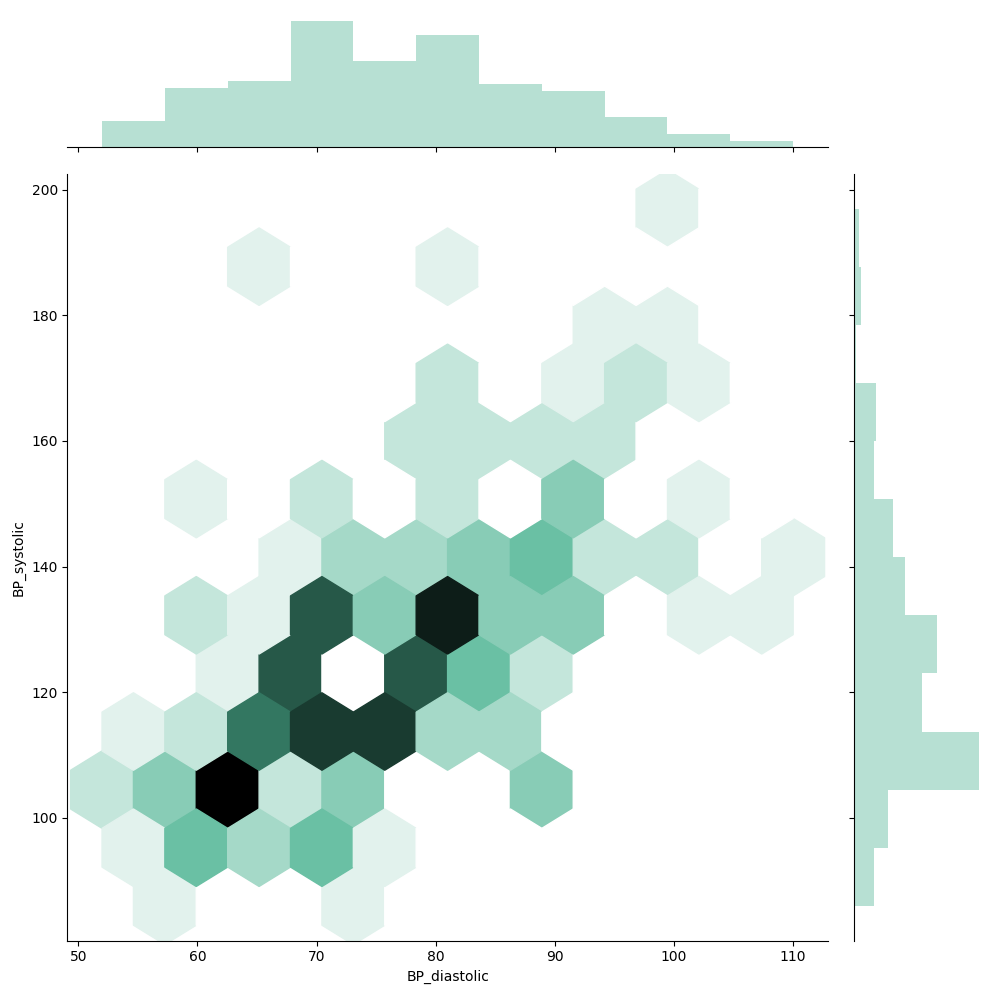
\includegraphics[width=0.4\textwidth]{data-exp/bp.png}
    \end{center}
    \caption{A joint distribtion plot of systolic and diastolic blood pressure of the patients.}
    \label{fig:bp-dist}
\end{figure}

Figure \ref{fig:meta-dist4} shows the patient distributions with regard to age, gender and \acrshort{bmi}. 
As evident from the figure the patients that make up the dataset is made up of 138 males and 57 females. 
The majority of the patients are in the age group 60-80 years with a number of patients in the range 80-90 years (AGE SECTION SUBJECT TO CHANGE). 
The \acrshort{bmi} distribution of patients is centered around 26 $kg/m^2$. 
Figure \ref{fig:bp-dist} shows the joint distribution of systolic and diastolic blood pressure among the patients. \bigskip

\section{Input variables} \label{sec:covariates}
As mentioned earlier in section REF the different machine learning models that will be applied will apply two types of input data, 
time-series data in the form of longitudinal strain curves, and point-values in the form of peak systolic global longitudinal strain and patient \acrshort{ef}. \bigskip

\subsection{Peak values}
As mentioned in section REFERENCE \acrshort{ef} values below 40-50$\%$ is regarded as unhealthy with regard to probability of heart failure. 
Keeping that in mind, one should note that the distribution of \acrshort{ef} values among the patients shown in figure \ref{fig:EF_dist} 
is centered at approximately 40$\%$ with tails going as low as 8$\%$ and as high as 70$\%$. 
Figure \ref{fig:gls_dist} shows the distribution of peak systolic \acrshort{gls} values, four the three different views. 
As evident from the figure, the values are centered around $-12.5$ with tails going as low as $-29$, and as high as $-2.5$. \bigskip

\begin{figure}[h]
    \begin{center}
    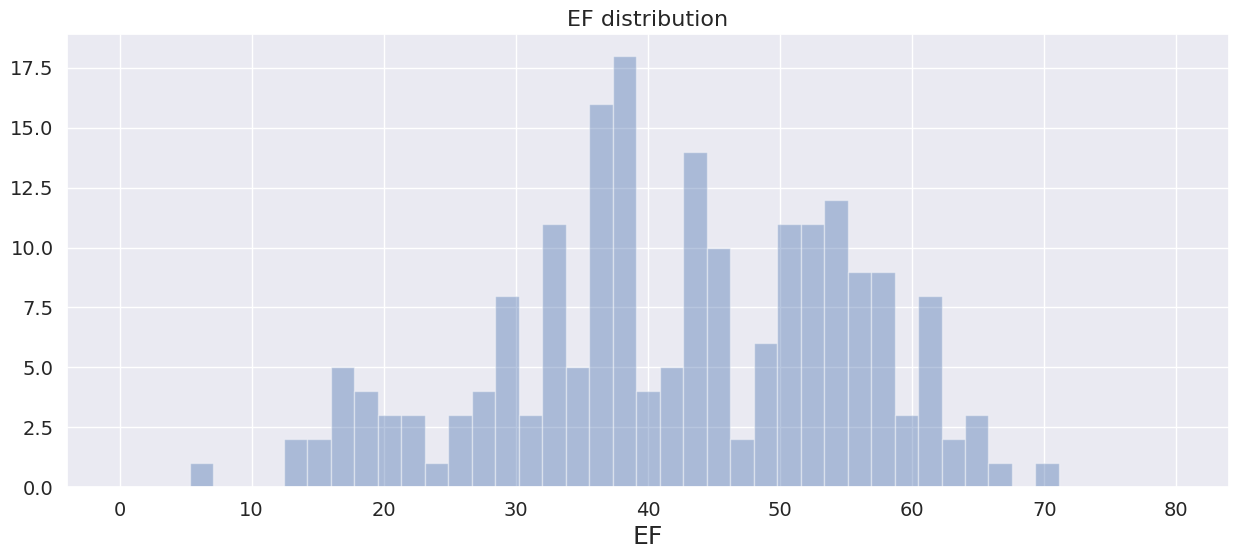
\includegraphics[width=\textwidth]{data-exp/EF_dist.png}
    \end{center}
    \caption{Distribution of patient \acrshort{ef} values.}
    \label{fig:EF_dist}
\end{figure}

\begin{figure}
    \begin{center}
    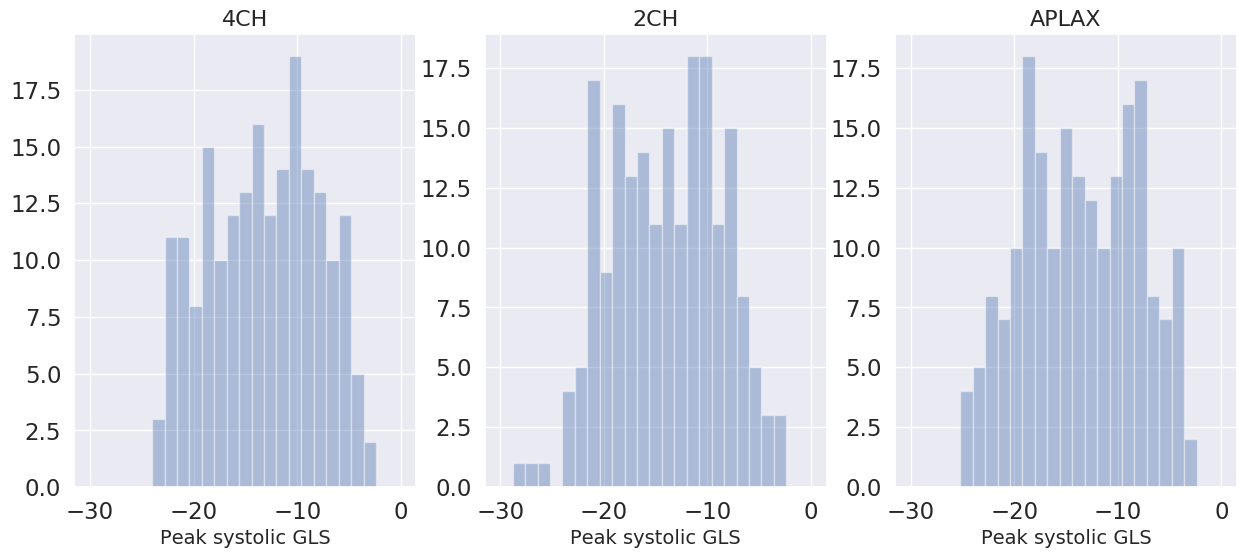
\includegraphics[width=\textwidth]{data-exp/peak_sys_gls_dist.png}
    \end{center}
    \caption{Distribution of peak systolic global longitudinal strain.}
    \label{fig:gls_dist}
\end{figure}

\subsection{Strain curves}
Figure \ref{fig:strain_curves} shows what a typical set of strain curves look like for a patient. 
Only the six regional strain curves, and the one global strain curve from the 4CH view have been included as they are fairly similar across the different views. 
Since the data from the different patients have been taken at different times, and possibly with different ultrasound machines 
factors such as number of samples per strain curve, and the frame rate of the particular ultrasound machine during an examination. 
Each strain curve has a standardized length of one heart cycle, due to this different curves have different number of samples. 
Figure \ref{fig:fr_sample_dist} shows the distribution of frame rates, and number of samples among the total number of strain curves. \bigskip

\begin{figure}[h]
    \begin{center}
    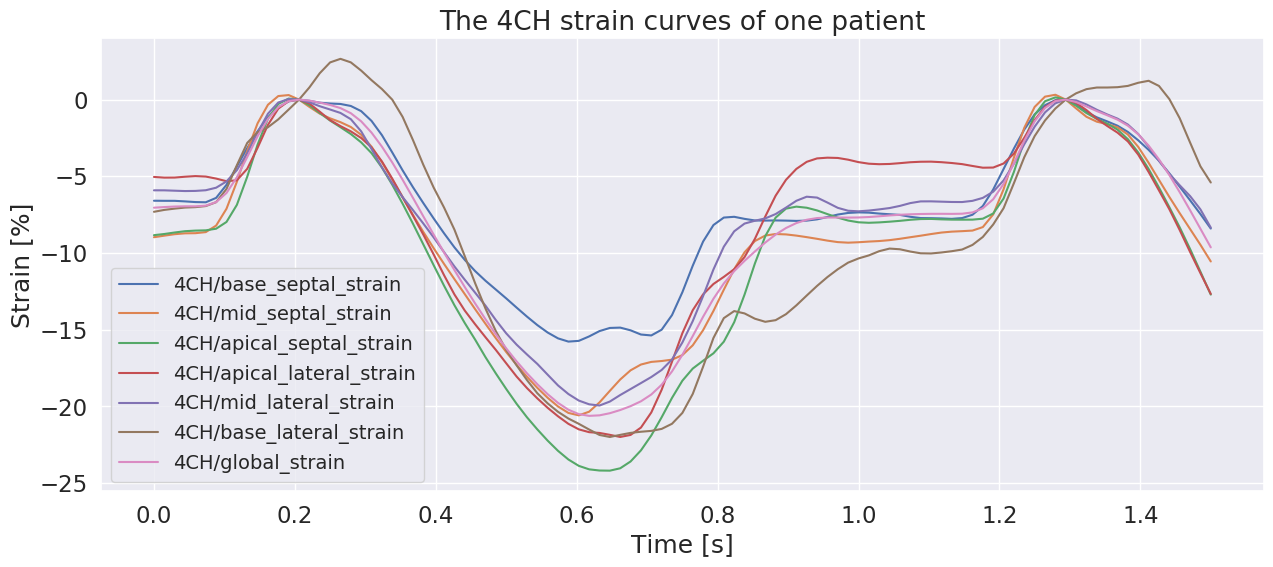
\includegraphics[width=0.95\textwidth]{data-exp/patient_strain_curves_4CH.png}
    \end{center}
    \caption{Plot of the global and regional longitudinal strain curves of one patient in the 4CH view.}
    \label{fig:strain_curves}
\end{figure}

\begin{figure}
    \begin{center}
    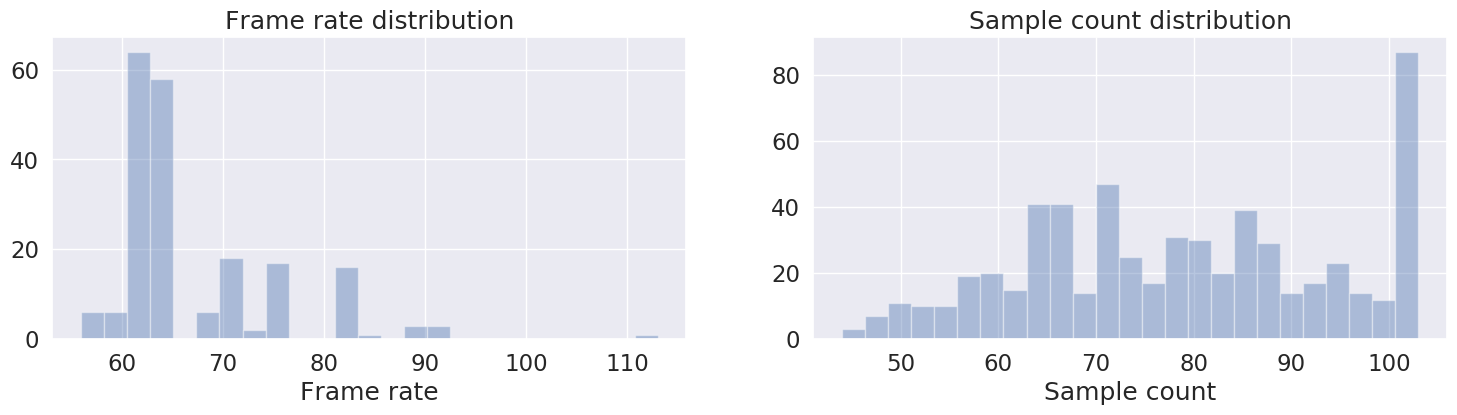
\includegraphics[width=\textwidth]{data-exp/fr_sample_dist.png}
    \end{center}
    \caption{Distribution of the frame rate used in the ultrasound imaging used to obtain the strain curves (left), and sample count of the different strain curves (right).}
    \label{fig:fr_sample_dist}
\end{figure}

\newpage

\section{Target variables} \label{sec:target}
Figure \ref{fig:hf_ind_dist} shows the distribution of heart failure among patients (left), and the distribution of different indications (right). 
Since the dataset has approximately as many patients with a heart failure diagnosis as without, it can be considered balanced in that regard. 
With regard to the different patient diagnosises, their rate of occurance can is not uniform in this dataset. 
The control group of healthy individuals consists of 31 patients. 
The groups of patients with STEMI, and NSTEMI indications consist of 60 and 39 patients respectively. 
Finally, the group of patients with heart failure, but with a non-stemic indication (labelled OTHER in left barplot in figure \ref{fig:hf_ind_dist}) consists of 69 patients. \bigskip

\begin{figure}[h]
    \begin{center}
    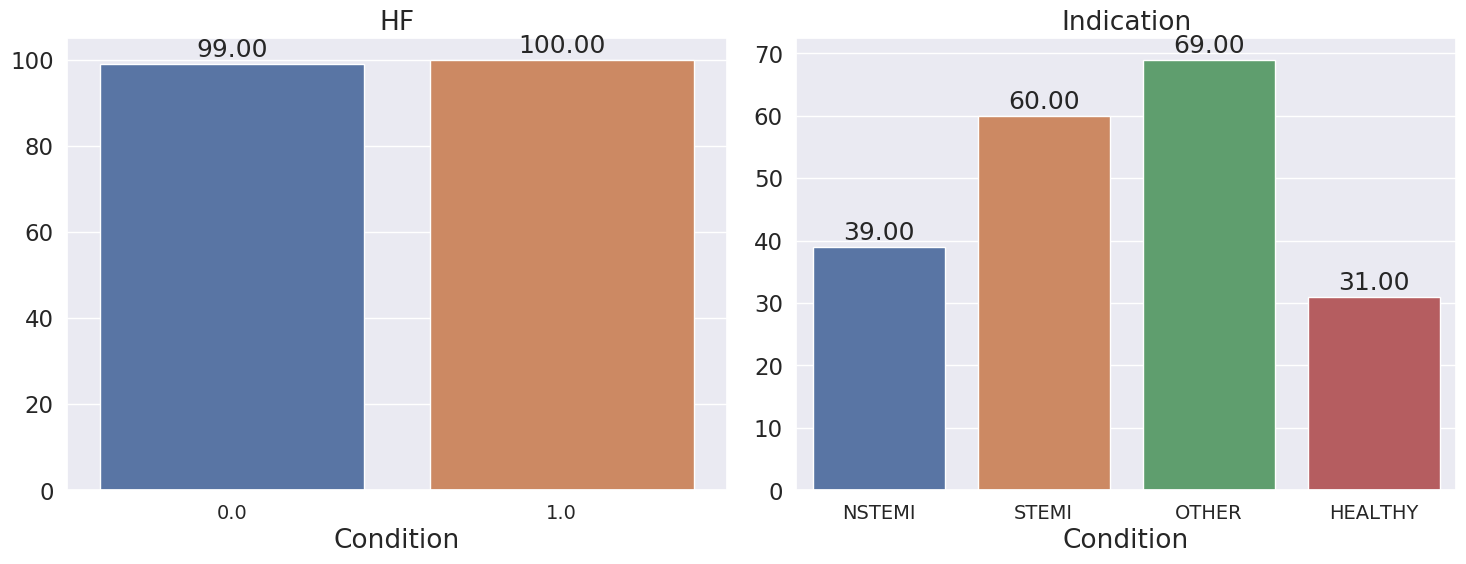
\includegraphics[width=\textwidth]{data-exp/hf_indication_dist.png}
    \end{center}
    \caption{The distribution of heart failure and different indications within patients.}
    \label{fig:hf_ind_dist}
\end{figure}

To illustrate the diagnostic power of \acrshort{ef}, and peak strain values figure \ref{fig:ef_hf_ind_dist} 
shows the distribution of \acrshort{ef} for patients with and without heart failure (left), and the distribution of \acrshort{ef} for patients in the control group and the other patients (right). 
Figure \ref{fig:gls_hf_dist} shows the distribution of peak systolic \acrshort{gls} values for patients with and without heart failure, 
and figure \ref{fig:gls_ind_dist} shows the distribution of peak systolic \acrshort{gls} values for patients in the control group and the rest of the patients. 
From the samples used to produce the left plot in figure \ref{fig:ef_hf_ind_dist} and figure \ref{fig:gls_hf_dist} 
it seems as though the heart failure patients are more separable with the \acrshort{ef} values than with the \acrshort{gls} values. 
With regard to separability of patients with diagnoses and patients in the control group it seems as though the right plot in figure \ref{fig:ef_hf_ind_dist}, 
and figure \ref{fig:gls_ind_dist} follows the same distribution as the heart failure patients. 
However, it is hard to make an evaluation on this since the sample size of the control group is much smaller than the group of diagnosed patients.\bigskip

\begin{figure}[h]
    \begin{center}
    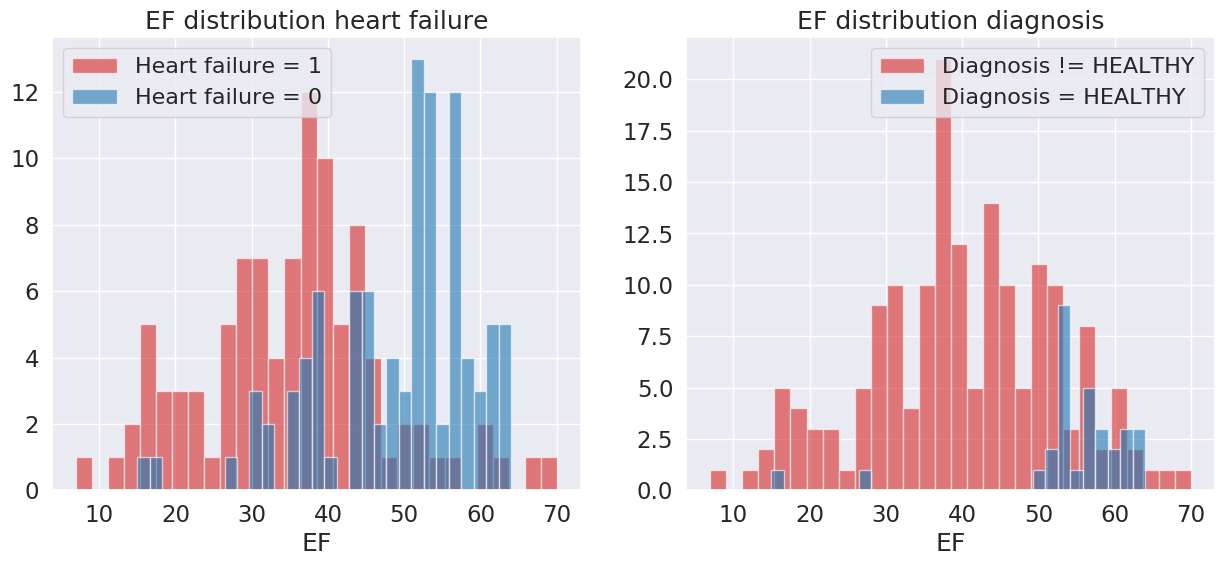
\includegraphics[width=\textwidth]{data-exp/EF_HF_ind_dist.png}
    \end{center}
    \caption{Distribution of \acrshort{ef} for patients with and without heart failure (left), and distribution of \acrshort{ef} for patients in the control group, and patients with a diagnosis.}
    \label{fig:ef_hf_ind_dist}
\end{figure}

\begin{figure}[h]
    \begin{center}
    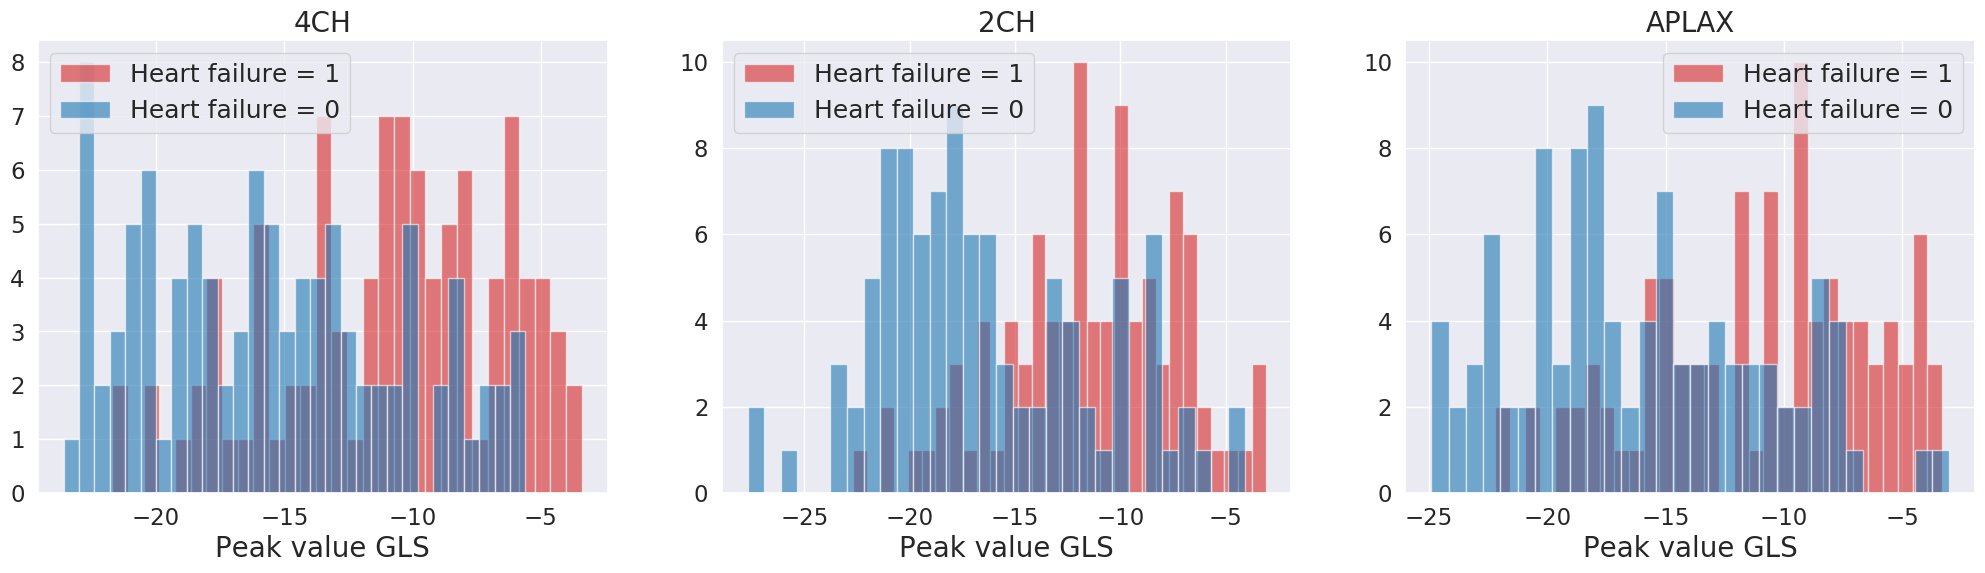
\includegraphics[width=\textwidth]{data-exp/gls_hf_dist.png}
    \end{center}
    \caption{Distribution of \acrshort{gls} for patients with and without heart failure.}
    \label{fig:gls_hf_dist}
\end{figure}

\begin{figure}[!h]
    \begin{center}
    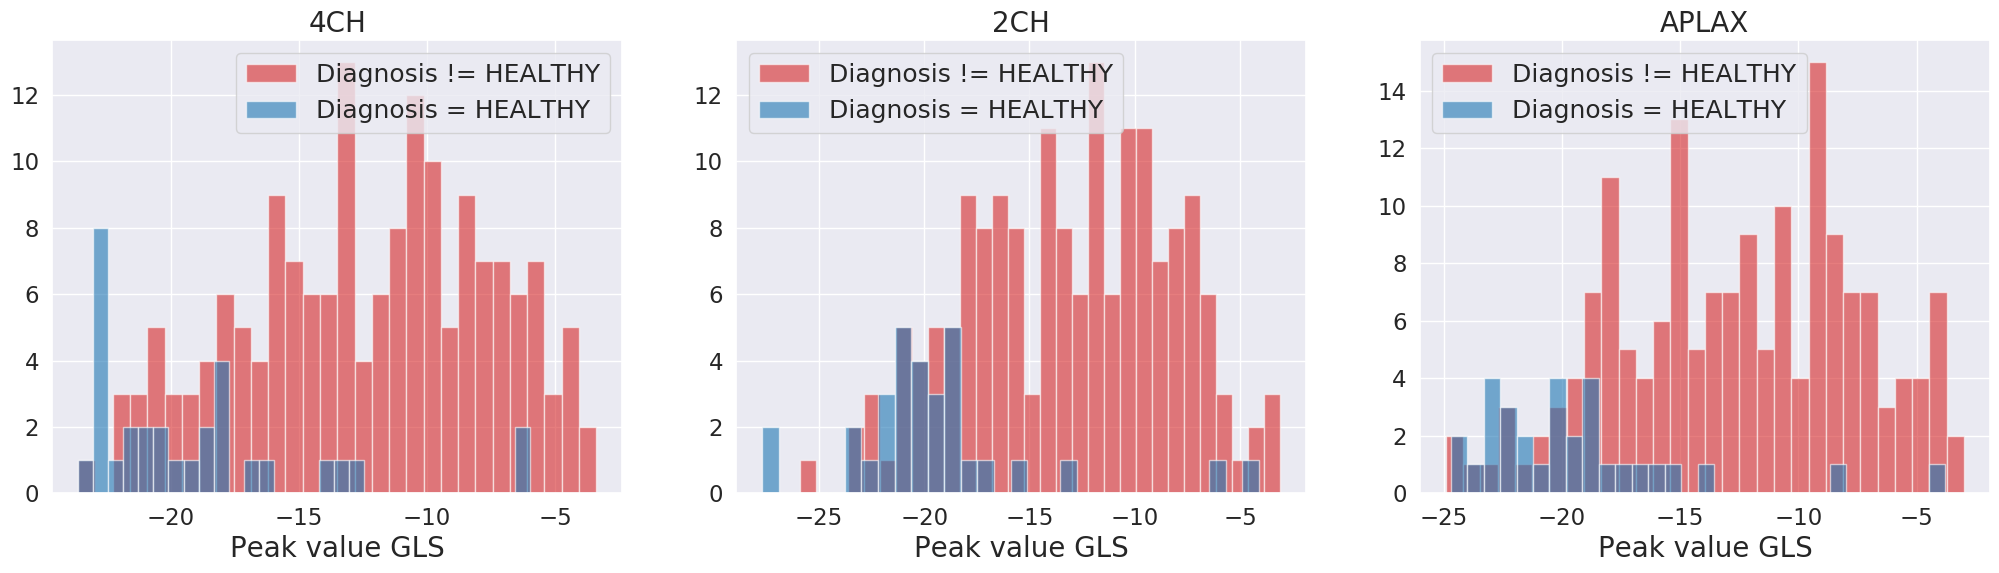
\includegraphics[width=\textwidth]{data-exp/gls_indication_dist.png}
    \end{center}
    \caption{Distribution of \acrshort{gls} for patients in the healthy control group, and the other patients.}
    \label{fig:gls_ind_dist}
\end{figure}

\newpage

Figure \ref{fig:segm_label_dist} shows the distribution of the different segment indications, for all the left ventricle segments of all the patients in the dataset. 
Since the occurance of indications other that ''normal'' and ''hypokinetic'' are very rare, the occurance axis has been used as logarithmic. 
The imbalance of segment-indication labels illustrated in figure \ref{fig:segm_label_dist} means that it will challenging for any statistical model 
to perform well in the classes with low occurance. 
To counteract this one can change the taxonomy of the labels such that the classification problem becomes binary with the labels \textit{Normal} and \textit{Not normal}. 
The dataset is then fairly evenly distributed with 1695 \textit{Normal} labels and 1818 \textit{Not normal} labels. \bigskip

\begin{figure}[!h]
    \begin{center}
    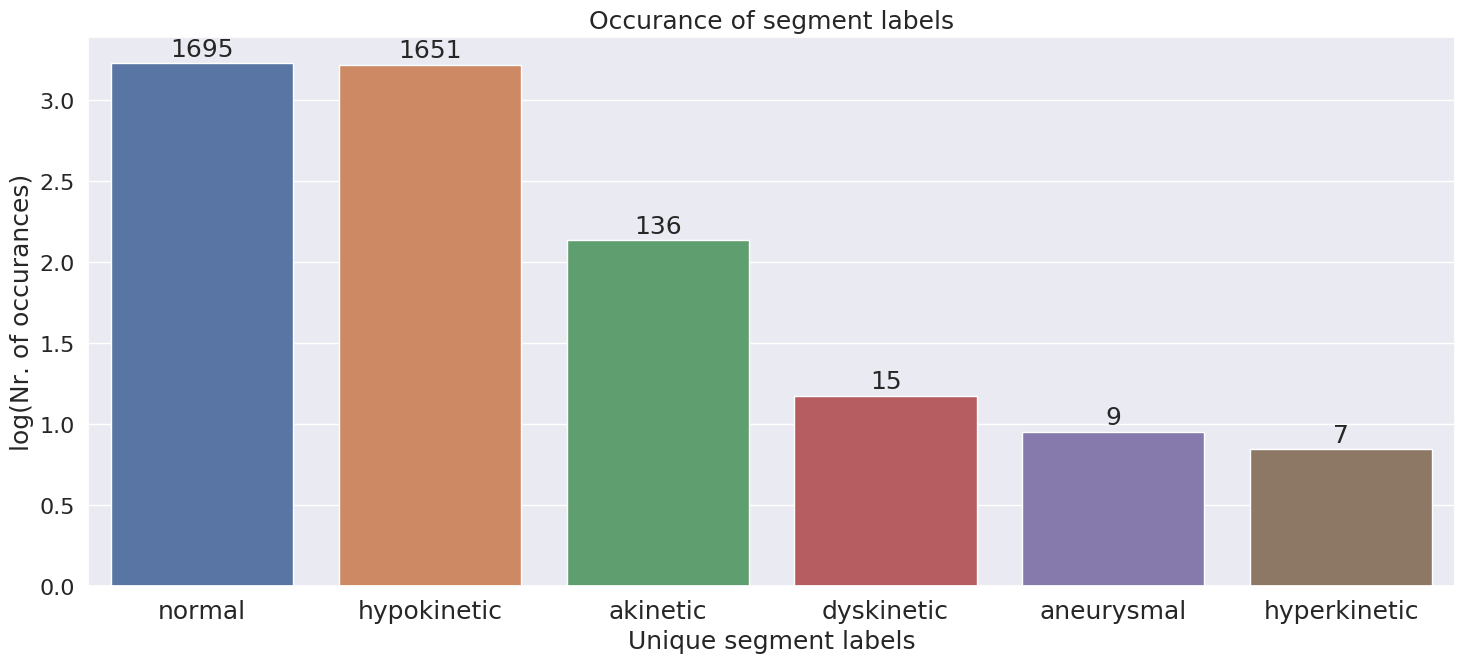
\includegraphics[width=\textwidth]{data-exp/segment_label_distribution.png}
    \end{center}
    \caption{Distribution segment indication labels.}
    \label{fig:segm_label_dist}
\end{figure}

